24. $\cfrac{x^2+9x+20}{(2x-x^2-1)(3x^2+x+2)}\leqslant0\Leftrightarrow \cfrac{(x+4)(x+5)}{-(x-1)^2\left(\left(x+\cfrac{1}{2}
ight)^2+2x^2+\cfrac{3}{4}
ight)}\leqslant0.$ Применив метод интервалов, найдём ответ: $x\in
(-\infty;-5]\cup[-4;1)\cup(1;+\infty).$
\begin{figure}[ht!]
\center{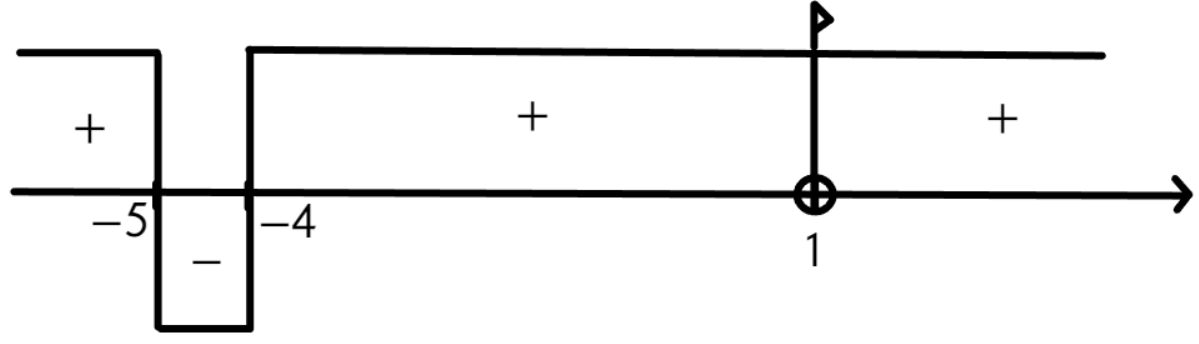
\includegraphics[scale=0.35]{ner9-24.png}}
\end{figure}
ewpage
oindent
